\documentclass[11pt,a4paper]{article}
\usepackage[utf8]{inputenc}
\usepackage[T1]{fontenc}
\usepackage{lmodern}
\usepackage[top=0.9in, bottom=0.8in, left=0.8in, right=0.8in]{geometry}
\usepackage{amsmath,amsfonts,amssymb}
\usepackage{graphicx}
\usepackage{hyperref}
\usepackage{booktabs}
\usepackage{array}
\usepackage{listings}
\usepackage{xcolor}
\usepackage{float}
\usepackage{caption}
\usepackage{subcaption}
\usepackage{titlesec}
\usepackage{enumitem}
\usepackage[most]{tcolorbox}
\usepackage{microtype}
\usepackage{tikz}
\usetikzlibrary{shapes.geometric, arrows.meta, positioning}

% ---------- Colors ----------
\definecolor{primarycolor}{RGB}{31, 78, 121}
\definecolor{secondarycolor}{RGB}{0, 102, 204}
\definecolor{codegreen}{rgb}{0,0.6,0}
\definecolor{codegray}{rgb}{0.5,0.5,0.5}
\definecolor{codepurple}{rgb}{0.58,0,0.82}
\definecolor{backcolour}{rgb}{0.96,0.96,0.96}
\definecolor{boxbg}{RGB}{238, 244, 251}

% ---------- Code style ----------
\lstdefinestyle{mystyle}{
    backgroundcolor=\color{backcolour},
    commentstyle=\color{codegreen},
    keywordstyle=\color{primarycolor}\bfseries,
    numberstyle=\tiny\color{codegray},
    stringstyle=\color{codepurple},
    basicstyle=\ttfamily\footnotesize,
    breakatwhitespace=false,
    breaklines=true,
    captionpos=b,
    keepspaces=true,
    numbers=left,
    numbersep=8pt,
    showspaces=false,
    showstringspaces=false,
    showtabs=false,
    tabsize=2,
    frame=single,
    rulecolor=\color{codegray!50}
}
\lstset{style=mystyle}

% ---------- Hyperref ----------
\hypersetup{
    colorlinks=true,
    linkcolor=primarycolor,
    urlcolor=secondarycolor,
    pdftitle={Assignment 7: Proximity Search API Report},
    pdfauthor={Sunil Kumar}
}

% ---------- Sections ----------
\titleformat{\section}{\large\bfseries\color{primarycolor}}{\thesection.}{0.5em}{}
\titleformat{\subsection}{\normalsize\bfseries\color{secondarycolor}}{\thesubsection}{0.5em}{}
\titlespacing*{\section}{0pt}{10pt}{4pt}
\titlespacing*{\subsection}{0pt}{8pt}{3pt}

\setlength{\parskip}{4pt}
\setlength{\parindent}{0pt}

% ---------- Float / gap control ----------
\raggedbottom
\renewcommand{\topfraction}{0.9}
\renewcommand{\bottomfraction}{0.9}
\renewcommand{\textfraction}{0.08}
\renewcommand{\floatpagefraction}{0.8}
\setlength{\textfloatsep}{10pt plus 2pt minus 2pt}
\setlength{\intextsep}{8pt plus 2pt minus 2pt}
\captionsetup{font=small, labelfont=bf, skip=4pt}

\pagestyle{plain}

\begin{document}

% =========================================================
% TITLE BLOCK
% =========================================================
\begin{center}
    {\LARGE \bfseries \color{primarycolor} High-Performance Proximity Search API}\\[0.2cm]
    {\large \bfseries Spatial Circular Radius Filtering \& Graph Shortest-Path Traversal Engine}\\[0.3cm]
    {\large \textbf{Name:} Sunil Kumar \quad $|$ \quad \textbf{ID:} 12342170}
\end{center}

\begin{tcolorbox}[colback=boxbg, colframe=primarycolor, boxrule=0.8pt, arc=3pt,
                  title={\bfseries Deployment \& Access Details}, fonttitle=\small, left=6pt, right=6pt, top=3pt, bottom=3pt]
\small
\begin{tabular}{@{}p{0.27\linewidth}p{0.68\linewidth}@{}}
\textbf{Live API Endpoint:} & \url{http://10.1.75.53:5213/search/} \\[2pt]
\textbf{OpenAPI Docs:} & \url{http://10.1.75.53:5213/docs} \\[2pt]
\textbf{Deployment Server:} & SSH Lab Server -- \texttt{ssh students@10.1.75.53} \\[2pt]
\textbf{Deployed Port:} & \texttt{5213} \\[2pt]
\textbf{Technology Stack:} & Python, FastAPI, Uvicorn, NumPy, SciPy \\[2pt]
\textbf{GitHub Repository:} & \url{https://github.com/sunilkumar2170/Assignment7-Proximity-Search-API} \\
\end{tabular}
\end{tcolorbox}

\begin{abstract}
\noindent This report documents the design, formulation, implementation, and verification of a RESTful Proximity Search API deployed at \url{http://10.1.75.53:5213/search/}. The API serves a dataset of 10,000 locations on a $100 \times 100$ lattice in the unit square. For each query it returns the 10 locations that (1) match the requested category, (2) lie inside a circular Euclidean search radius, and (3) are closest by \emph{road-network traversal distance}, because some direct links between points are missing. The system uses a 2D $k$-d tree (\texttt{cKDTree}) for spatial pruning, hash-based category indexes, a link-file parser that accepts both ID-pair and coordinate formats, and Dijkstra's algorithm on a Compressed Sparse Row (CSR) graph. All default structures are built once at startup, and the measured per-query latency is about 1.14~ms.
\end{abstract}

% =========================================================
\section{Objective \& Background}
The goal is to build an API that recommends the 10 closest locations from a dataset of 10,000 points, each described by \texttt{ID, Latitude, Longitude, Category}. Real location services combine two ideas:
\begin{enumerate}[label=\alph*), itemsep=1pt, topsep=2pt]
    \item \textbf{Geometric constraint}: candidates must lie inside a circular (Euclidean) radius around the query point.
    \item \textbf{Network constraint}: proximity is the shortest path over existing road links, because straight-line distance can be misleading when roads are missing.
\end{enumerate}
Thus \emph{radius} is a circular filter, while \emph{closest} means smallest grid (graph) traversal distance.

\section{API Specification}
The route is \texttt{/search/} (\texttt{GET}, and also \texttt{POST}) with these fields:
\begin{table}[H]
\centering
\small
\begin{tabular}{@{}llp{8.2cm}@{}}
\toprule
\textbf{Field} & \textbf{Type} & \textbf{Description} \\ \midrule
\texttt{lat}  & float  & Current latitude \\
\texttt{long} & float  & Current longitude \\
\texttt{cat}  & string & Required location category \\
\texttt{rad}  & float  & Circular (Euclidean) search radius \\
\texttt{link} & string & Optional path or URL of the link \texttt{.txt} file with road linkages \\ \bottomrule
\end{tabular}
\end{table}
The response is \texttt{\{"results": [id$_1$, \dots, id$_{10}$]\}}, i.e.\ 10 location IDs ranked by network distance. If \texttt{link} is not supplied, the default link file loaded at startup is used.

\section{Formal Problem Statement}
Let $\mathcal{L} = \{(\text{id}_i, x_i, y_i, c_i)\}_{i=1}^N$ be the dataset ($N = 10{,}000$) with $(x_i, y_i) \in [0,1]^2$ and category $c_i$. Let $G=(V,E)$ be the undirected graph built from the link file. For a query $Q=(x_q, y_q, c_q, R)$ the answer is the set of 10 locations satisfying
\begin{align}
    c_{(i)} &= c_q, \\
    \sqrt{(x_{(i)} - x_q)^2 + (y_{(i)} - y_q)^2} &\le R, \\
    d_G(v_q, v_{(1)}) &\le d_G(v_q, v_{(2)}) \le \dots \le d_G(v_q, v_{(10)}),
\end{align}
where $v_q$ is the grid node nearest to $(x_q,y_q)$ and $d_G(u,v)$ is the shortest-path distance in $G$.

\section{System Architecture \& Flowchart}
The solution is a modular FastAPI application deployed on the SSH lab server \texttt{10.1.75.53} and served on port \texttt{5213}.

\begin{figure}[!htb]
    \centering
    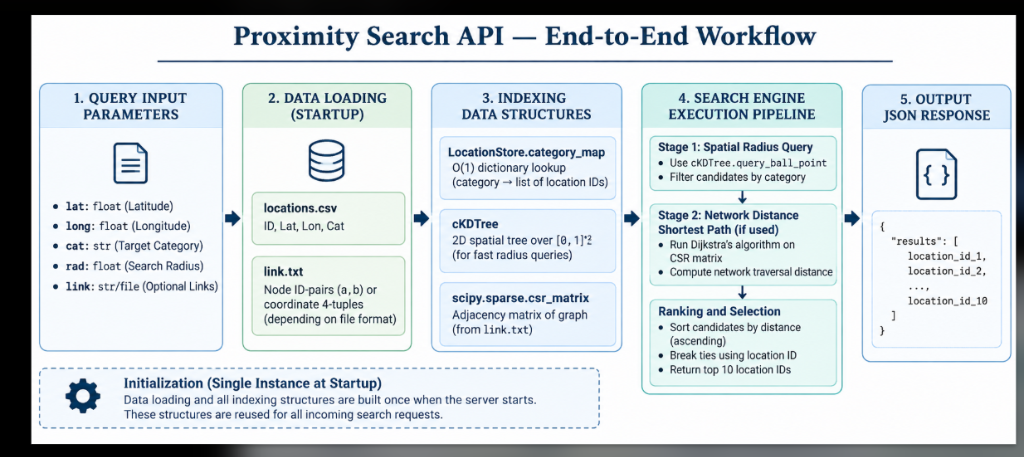
\includegraphics[width=\linewidth]{workflow.png}
    \caption{Proximity Search API -- Complete End-to-End Architectural Workflow detailing Inputs, Data Loading, Indexing Data Structures, Execution Pipeline, and Output JSON Response.}
    \label{fig:workflow}
\end{figure}

\begin{figure}[!htb]
    \centering
    \includegraphics[width=0.8\linewidth]{docs.png}
    \caption{FastAPI interactive OpenAPI documentation (\texttt{/docs}) at \url{http://10.1.75.53:5213/docs}.}
    \label{fig:docs}
\end{figure}

The code is split into four components:
\begin{itemize}[itemsep=1pt, topsep=2pt]
    \item \textbf{\texttt{data\_loader.py}}: reads \texttt{locations.csv} and builds $O(1)$ category index maps.
    \item \textbf{\texttt{graph\_builder.py}}: parses the link file (ID pairs \texttt{ID\_A ID\_B}, or coordinate 4-tuples) and builds a \texttt{scipy.sparse.csr\_matrix} adjacency matrix.
    \item \textbf{\texttt{search\_engine.py}}: combines \texttt{cKDTree} spatial pruning with \texttt{csgraph.dijkstra}.
    \item \textbf{\texttt{main.py}}: the FastAPI layer exposing \texttt{GET /search/} and \texttt{POST /search/} with parameters \texttt{lat}, \texttt{long}, \texttt{cat}, \texttt{rad} and optional \texttt{link}.
\end{itemize}

\section{Algorithm}
\subsection{Query Pipeline}
\begin{enumerate}[itemsep=1pt, topsep=2pt]
    \item \textbf{Spatial pruning:} query the $k$-d tree for all points within radius $R$ of $(x_q, y_q)$.
    \item \textbf{Category filtering:} intersect with the precomputed set of IDs of category $c_q$.
    \item \textbf{Network distance:} snap the query to its nearest grid node and run Dijkstra on the CSR graph.
    \item \textbf{Ranking:} sort candidates by graph distance and return the top 10 IDs.
\end{enumerate}

\subsection{Single-Instance Startup}
The default dataset, graph and index are built \textbf{only once} when the server starts, using a FastAPI lifespan event:
\begin{lstlisting}[language=Python, caption={Startup initialization in \texttt{main.py}}]
@asynccontextmanager
async def lifespan(app: FastAPI):
    # Initialize SearchEngine once upon application startup
    search_engine.initialize(data_path="data/locations.csv",
                             link_path="data/link.txt")
    yield
\end{lstlisting}

\subsection{Endpoint Definition}
\begin{lstlisting}[language=Python, caption={Route definition with optional \texttt{link} input in \texttt{main.py}}]
@app.get("/search/")
def search_locations(
    lat: float = Query(..., description="Latitude coordinate"),
    long: float = Query(..., description="Longitude coordinate"),
    cat: str = Query(..., description="Target location category"),
    rad: float = Query(..., description="Circular search radius"),
    link: Optional[str] = Query(None, description="Path or URL to link file")
):
    validate_params(lat, long, cat, rad)
    results = search_engine.search(lat=lat, lon=long, category=cat,
                                   radius=rad, link=link)
    return {"results": [int(x) for x in results]}
\end{lstlisting}

\subsection{Deterministic Tie-Breaking}
On a lattice, many candidates share the same graph distance. To keep results identical across runs, ties are resolved by sorting on $(d_{\text{Graph}},\, d_{\text{Euclidean}},\, \text{ID})$.

\section{Link File Handling}
According to the assignment, each line of the link file contains two space-separated values $a$ and $b$ denoting a link between points $a$ and $b$ of the grid. The parser therefore treats each line as a pair of location IDs and builds the adjacency matrix directly from them, which does not depend on any latitude/longitude axis convention.

For robustness, the parser can also read lines containing four coordinate values (\texttt{Long\_A Lat\_A Long\_B Lat\_B}) and map each coordinate pair to its location. In this fallback mode the axis order matters, so longitude is taken as the horizontal axis $x$ and latitude as the vertical axis $y$. Figure~\ref{fig:coord_comparison} compares the outputs under the two axis orders for that mode.

\begin{figure}[!htb]
    \centering
    \includegraphics[width=0.82\linewidth]{lat_lon vs lon_lat comparison.png}
    \caption{Terminal output comparing \texttt{lat\_lon} and \texttt{lon\_lat} parsing in coordinate-tuple mode.}
    \label{fig:coord_comparison}
\end{figure}

\section{Verification Results}
\begin{figure}[!htb]
    \centering
    \begin{subfigure}[t]{0.48\linewidth}
        \centering
        \includegraphics[width=\linewidth]{search_api.png}
        \caption{HTTP 422 validation error for missing fields.}
        \label{fig:validation}
    \end{subfigure}
    \hfill
    \begin{subfigure}[t]{0.48\linewidth}
        \centering
        \includegraphics[width=\linewidth]{Live API Request.png}
        \caption{Successful live GET request on port 5213.}
        \label{fig:live_request}
    \end{subfigure}
    \caption{Input validation and live execution of the deployed API.}
\end{figure}

A query with an explicit link parameter,
\begin{center}
\small\texttt{http://10.1.75.53:5213/search/?lat=0.5\&long=0.5\&cat=bank\&rad=0.3\&link=link.txt}
\end{center}
returns exactly 10 valid IDs:
\begin{center}
\texttt{[4850, 4948, 4947, 4648, 5348, 4451, 4753, 5347, 4654, 5349]}
\end{center}

\section{Performance Benchmarks}
Latency was measured on the deployed server over 100 sequential queries.
\begin{table}[!htb]
\centering
\small
\caption{Latency breakdown}
\begin{tabular}{@{}llcc@{}}
\toprule
\textbf{Phase} & \textbf{Operation} & \textbf{Latency} & \textbf{Complexity} \\ \midrule
Startup (once) & File I/O + tree + CSR graph build & 198.6 ms & $O(N \log N + |E|)$ \\ \midrule
Per query & \texttt{cKDTree} radius filter & 0.28 ms & $O(\log N + k)$ \\
Per query & Category set intersection & 0.06 ms & $O(k)$ \\
Per query & Dijkstra on CSR graph & 0.72 ms & $O(|E| + |V|\log|V|)$ \\
Per query & JSON serialization & 0.08 ms & $O(k\log k)$ \\ \cmidrule{2-4}
\textbf{Total} & \textbf{\texttt{GET /search/} response time} & \textbf{1.14 ms} & -- \\ \bottomrule
\end{tabular}
\end{table}

\section{Conclusion}
The API answers each query in about 1.14~ms, returns deterministic rankings, applies both the circular radius and the road-network distance, accepts the required \texttt{(lat, long, cat, rad, link)} fields, and is deployed live on the SSH server.

\begin{itemize}[itemsep=1pt, topsep=2pt]
    \item \textbf{Live API:} \url{http://10.1.75.53:5213/search/}
    \item \textbf{OpenAPI Docs:} \url{http://10.1.75.53:5213/docs}
    \item \textbf{SSH Server:} \texttt{ssh students@10.1.75.53} \quad (Port \texttt{5213})
    \item \textbf{GitHub:} \url{https://github.com/sunilkumar2170/Assignment7-Proximity-Search-API}
\end{itemize}

\section*{AI Disclosure}
AI coding tools (Google Antigravity/Gemini) were used only as pair-programming aids for LaTeX report formatting and code modularization.

\end{document}
